\documentclass[times, utf8, zavrsni]{fer}
\usepackage{booktabs}

\begin{document}

% TODO: Navedite broj rada.
\thesisnumber{920}

% TODO: Navedite naslov rada.
\title{Web-aplikacija za praćenje podataka o nogometnim utakmicama.}

% TODO: Navedite vaše ime i prezime.
\author{Marko Jerkić}

\maketitle

% Ispis stranice s napomenom o umetanju izvornika rada. Uklonite naredbu \izvornik ako želite izbaciti tu stranicu.
% TODO: Treba li mi izbornik?
% \izvornik

% Dodavanje zahvale ili prazne stranice. Ako ne želite dodati zahvalu, naredbu ostavite radi prazne stranice.
\zahvala{}

\tableofcontents

\chapter{Uvod}
Uvod rada. Nakon uvoda dolaze poglavlja u kojima se obrađuje tema.
Test uvod.

\chapter{Analiza postojećih rješenja na internetu}
Za analizu postojećih rješenja na internetu su korištene aplikacije Sofascore\footnote{https://sofascore.com}, OneFootball\footnote{https://onefootball.com} i Rezultati.com\footnote{https://rezultati.com}.

\section{Prikaz liste utakmica}

Jedan od glavnih dijelova aplikacija koje se koriste za praćenje nogometnih rezultata je stranica pregleda popisa dostupnih utakmica.
Većina postojećih rješenja na internetu koriste ovu stranicu kao središnju lokaciju s kojih se pregleda većina sadržaja. To je istina za aplikacije Sofascore i Rezultati.com.

U slučaju te dvije aplikacije, prilikom pristizanja na samu web-lokaciju, prikazana nam je lista postojećih utakmica koje se igraju na dan posjećivanja aplikacije.

Središnja komponenta početne stranice Sofascore-a je lista utakmica grupirana po natjecanjima i državama. Prvih nekoliko prikazanih natjecanja su istaknuta ili spremljena natjecanja.
U slučaju kada korisnik prvi put posjećije stranicu ili nema spremljenih podataka u pregledniku, istaknuta natjecanja uključuju velika svjetska natjecanja,
kao engleska Premier liga, njemačka Bundesliga i slično te velika natjecanja u državi iz koje korisnik posjećuje stranicu.
Za korisnika koji posjećuje stranicu iz Hrvatske, među istaknutim natjecanjima se nalazi Hrvatska nogometna liga.
Nakon istaknutih natjecanja, prikazuju se natjecanja iz cijelog svijeta koja sadrže utakmice za odabrani dan. Natjecanja su grupirana po državama u kojima se održava to natjecanje.

Osim popisa utakmica, koji se nalazi u sredini aplikacije, Sofascore sadrži kalendar s lijeve strane popisa utakmica.
Kalendar se koristi za odabir datuma prema kojemu se prikazuju dostupne utakmice.
Ispod kalendara se nalazi popis istaknutih natjecanja i popis svih dostupnih natjecanja s poljem za unos teksta koji se koristi za sužavanje izbora.

S desne strane popisa utakmica se nalazi pretpregled istaknute utakmice. Pretpregled sadrži ime i grb ekipa koje su sudjelovale u utakmici te rezultat utakmice.
Ispod toga se nalazi popis istaknutih igrača te reklame za sportsko klađenje.

Aplikacija Rezultati.com ima dosta sličan raspored na početnoj stranici, ali ne prikazuje istaknuta natjecanja, utakmice niti igrače.
Aplikacija OneFootball ne koristi popis dostupnih utakmica na početnoj stranici. OneFootball je aplikacija koja se fokusira prvenstveno na nogometne novosti.
Do stranice na kojoj se prikazuje popis dostupnih utakmica se dolazi preko poveznice koja se nalazi u navigacijskoj traci.

\section{Prikaz detalja utakmice}

Sve tri aplikacije koje su korištene za analizu postojećih rješenja imaju dosta različito ponašanje prilikom odabira utamice s popisa.
Prilikom odabira utakmice na aplikaciji Sofascore otvori se pretpregled desno od popisa utakmica.
Aplikacija Rezultati.com otvori detalje utakmice u skočnom prozoru, dok OneFootball otvori novu stranicu.

Zaglavlje stranice detalja utakmice prikazuje ime i grb ekipa koje su sudjelovale u utakmici, datum utakmice i trenutni rezultat.
Detaljni podatci su raspodijeljeni u više kategorija koje se odabiru preko kartica. Zadana kartica sadrži događaje utakmice, kao što su pogodci, kartoni i zamjene, kronološki poredane po minuti.

Pored kartice događaja po minuti, bitne su još kartica početnih postava dviju ekipa te kartica statistike utakmice.
Kartica početnih postava utakmice grafički prikazuje prvih jedanaest igrača obje ekipe, formaciju, boju dresova te broj na dresovima.
Kartica statistike prikazuje podatke o posjedu lopte, broju udaraca, broju udaraca u vrata, broju udaraca iz kuta i sl., za obje ekipe.

\section{Prikaz detalja igrača, izbornika, ekipa i natjecanja}

Nakon stranica prikaza popisa utakmica i detalja pojedinačne utakmice, sporednu ulogu u odabranim aplikacijama zauzimaju stranice pregleda detalja igrača, izbornika, ekipa i natjecanja.

Stranice pregleda detalja igrača i izbornika su dosta slične. Obje prikazuju ime osobe, sliku, datum rođenja i nacionalnost.
Ispod toga se prikazuju kartice s popisom najnovijih utakmica u kojima je sudjelovala ta osoba, osobna statistika te popis ekipa za koje je ta osoba igrala ili koje je ta osoba trenirala.

Stranica prikaza detalja o ekipi prikazuje ime ekipe, grb i državu iz koje dolazi. Nakon toga se prikazuju kartice s podatcima o nedavnim utakmicama koje je igrala ekipa,
trenutnim igračima koji igraju za tu ekipu, te tablica poretka natjecanja u kojemu ta ekipa sudjeluje.

Kod stranice pregleda natjecanja, najbitnije su kartice s tablicom poretka te popisom utakmica po sezoni za odabrano natjecanje.

\chapter{Relacijski model baze podataka}

Dizajnirani relacijski model podataka sadrži 19 tablica te 6 enumeracijski vrsti.

Središnji entitet relacijskog modela je tablica "Game," koja sadrži osnovne podatke o utakmici. Ovaj entitet sadrži veze na natjecanje kojemu pripada utakmica, domaću i gostujuću ekipu, izbornika domaće i gostujuće ekipe,
sezonu u kojoj se igra utakmica te na tablicu koja sarži detaljniju statistiku utakmice. Tablica "Game" sadrži foreign key na tablicu "GameStatistic," ali taj podatak nije obavezan jer svaka utakmica ne mora imati podatke o statistici.
U slučaju kada utakmica još nije počela, entitet "Game" ne sadrži podatke o statistici, pa to polje sadrži vrijednost "null."

Entitet "Game" također sadržava informaciju o vremenu početka utakmice, vremenu nadoknade u prvom i drugom poluvremenu, boju dresova domaće i gostujuće ekipe, kao i boje dresova vratara, status utakmice, te početne postave dviju ekipa.
Status utakmice se sprema kao enumirana vrijednost koja može poprimiti vrijednosti "NOT\textunderscore STARTED," "STARTED," "HALFTIME" te "OVER".

Početne postave prvih jedanaest se spremaju kao "jsonb"\footnote{https://www.postgresql.org/docs/9.5/functions-json.html} \citep{postgressjson} vrsta podataka.
Podatci se spremaju kao JSON polje od jedanaest vrijednosti koje predstavljaju jedanaest igrača početne postave. U tom JSON podatku je spremljen identifikator igrača, broj dresa koji igrač nosi na toj utakmici, broj reda u početnoj formaciji te redni broj igrača u tome redu gledajući s lijeva na desno.
Odlučeno je spremati početnu postavu kao JSON vrijednost umjesto da se stvori novi entitet koji bi imao vezu na entitet "Game" jer bi to stvorilo previše unosa u bazi podataka, točnije 22 po svakoj spremljenoj utakmici.
Pored toga, spremanje tog podatka kao JSON je olakšalo način izrade administracije početne postave kroz klijetsku aplikaciju.

Entitet "GameStatistics" sadrži podatke kao ukupni udarci, udarci u vrata, ubačaji iz kuta, prekršaji, stvorene velike prilike, broj dodavanja, broj ubacivanje lopte u šesnaesterac, broj driblinga i broj uklizavanja za obje ekipe.

Pored nabrojanih podataka iz entiteta "GameStatistics," izdvojeni su podatci o zabijenim pogotcima, podijeljenim kartonima te zamijenama kao posebni entiteti. Razlog tomu je taj što svi ovi podatci sadrže bar jednu vezu na nekog igrača.
Entitet "Goal" sadrži podatak o igraču koji je zabio pogodak, o igraču koji je asistirao te vrijeme u minutama kada je zabijen pogodak. Entitet "CardAwarded" sadrži igrača koji je dobio karton, minutu u kojoj je igrač dobio karton, te vrstu kartona koji je dodijeljen.
A entitet "Substitution" sadrži igrača koji je izašao s terena, igrača koji ulazi u teren te minutu u kojoj je zamjena izvršena.

Svaka utakmica pripada jednom natjecanju u određenoj sezoni. Entitet "Competition" sadrži ime, podatak o državi u kojoj se igra te podatak o tome jeli to natjecanje označeno kao istaknuto.
Država u kojoj se igra natjecanje je spremljena kao poseban entitet koji sadrži naziv države te poveznicu na sličicu zastave te države.
Svako natjecanje može imati više sezona, te za jednu sezonu može postojati više natjecanja. Sezona je spremljena kao vlastiti entitet i jedini podatak koji sadrži, pored identifikatora, je naziv te sezone.

Entiet "Team" sadrži podatke o nazivu ekipe, državi iz koje potječe klub te poveznicu na sličicu grba ekipe. Entitet "Team" sadrži više-na-više vezu s poveznom tablicom "CompetitionInSeason" koja sadrži vezu na jedno natjecanje i sezonu.

Entiteti "Manager" i "Player" su dosta slični. Oba sadrže ima, prezime, datum rođenja, trenutnu ekipu (koja nije obavezna) te nacionalnost. Oba imaju više-na-više vezu s poveznom tablicom "TeamInCompetition" koja sadrži podatak o ekipi koja igra u određenom natjecanju u određenoj sezoni.
To znači da jedan izbornik ili igrač može pripadati više ekipa u jednoj sezoni, ali također ne mora pripadati niti jednoj ekipi za određenu sezonu.

Pored nabrojanih entiteta postoje još entiteti potrebni za autentifikaciju te spremanje najdražih igrača i ekipa korisnika.

\chapter{Odabrane tehnologije i arhitektura}

Arhitektura aplikacije se sastoji od NodeJS\footnote{https://nodejs.org/en} koja obrađuje HTTP zahtjeve te poslužuje statični sadržaj (kao HTML, JavaScript i CSS datoteke) i dinamične podatke u obliku JSON-a te PostreSQL\footnote{https://www.postgresql.org/} baze podataka.

\section{Backend i frontend tehnologija}
NodeJS aplikacija je napisana koristeći meta-framework SolidStart\footnote{https://start.solidjs.com}. Meta-framework \citep{meta2022davanzo} je software koji je napisan da upotpuni neki postojeći frontend framework.
Većim meta-framework propisuje načine na koji se radi dohvat i pisanje podataka te donosi vlastiti usmjerivač\footnote{https://hr.wikipedia.org/wiki/Usmjerivač} (eng. router).

SolidStart je meta-framework oko popularnog frontend framework-a SolidJS\footnote{https://solidjs.com}. SolidJS je postao popularan u poljednjih nekoliko godina zbog svog modela reaktivnosti klijentskih JavaScript aplikacija.
SolidJS je obnovio ideju signala stanja. Ryan Carniato \citep{ryan2023signal} opisuje signal kao reaktivno stanje aplikacije kojemu se pristupa preko observer obrazca\footnote{https://en.wikipedia.org/wiki/Observer\_pattern}.
Stanje se drži u jednom objektu i može se dijeliti na više mjesta. Na svakom mjestu gdje se želi pristupiti tome stanju potrebno je se pretplatiti na izvor signala. To se učini tako da se pozove funkcija signala.
Svagdje gdje se pozove funkcija signala automatski se pretplati na sami izvor.
Najveća prednost signala je ta što je moguće pretplititi JavaScript DOM\footnote{https://developer.mozilla.org/en-US/docs/Web/API/Document\_Object\_Model/Introduction} na signal.
To znači da svaki put kada se u signal upiše nova vrijednost, izvornik pošalje obavijest svim pretplaticima te ako je DOM među pretplatnicima, SolidJS runtime preuzme najnoviju vrijednost tog signala te izmjeni samo
one čvorove HTML stabla koji su pretplaćeni na njega.

Ovaj način ažuriranja HTML stabla je jako efikasan. U prosjeku mu treba manje vremena da ažurira HTML stablo od frameworka kao React\footnote{https://react.dev} koji koriste virtualni DOM\footnote{https://legacy.reactjs.org/docs/faq-internals.html} na koji se pišu sve promjene te usporede virtualni i stvarni DOM pa se ažuriraju samo promijenjeni čvorovi.
SolidJS time također rezultira manjim prevedenim JavaScript datotekama jer ne mora s njima slati cijeli virtualni DOM.
Ovaj način ažuriranja HTML stabla je poznat kao "fine-grained reactivity"\citep{ryan2021reactivity}.

\section{Poslužitelj}
Aplikacija se poslužuje na poslužitelju Vercel\footnote{https://vercel.com}. Aplikacije se poslužuje koristeći tvz. "bezposlužiteljsku" (eng. serverless).
To znači da postoji jedan poslužitelj koji konstantno vrti aplikaciju i čeka zahtjeve. Svaki put kada dođe novi zahtjev, provjeri se postoji li uključena Lambda\footnote{https://aws.amazon.com/lambda/} instanca, a ako ne postoji onda se pokrene nova, i onda ta instanca obradi zahtjev.
Ako nakon nekoliko minuta ta lambda instanca ne dobije novi zahtjev, onda se ona ugasi \citep{serverless2022}.

Baza podataka koristi poslužitelj Supabase\footnote{https://supabase.com/} gdje je pokrenuta instanca PostreSQL servera.
Supabase se također koristi za obavijsti o promjenama podataka određenih entiteta u bazi na osnovu kojih se na klijentu ažuriraju podatci u stvarnom vremenu.

Aplikacija je poslužena pod domenom \emph{https://football.jerkic.dev}.

\chapter{Izrada aplikacije}

\section{Autentifikacija}

Od korisnika se očekuje da bude autentificiran za samo jednu funkcionalnost, a to je spremanje omiljenih igrača i ekipa. Korisnik koji označi nekog igrača ili ekipu kao omiljenu brže može pronaći podatke o utakmicama i statistici te ekipa ili igrača.

Svakom korisniku na navigacijskoj traci je prikazana tipka koja vodi do korisničkog profila. Ako korisnik nije prijavljen, onda aplikacija zatraži od njega da se prijavi tako da ga prebaci na odgovarajuću putanju.

Ekran za prijavu u sustav traži od korisnika korisničko ime i zaporku.

\begin{figure}[htb]
\centering
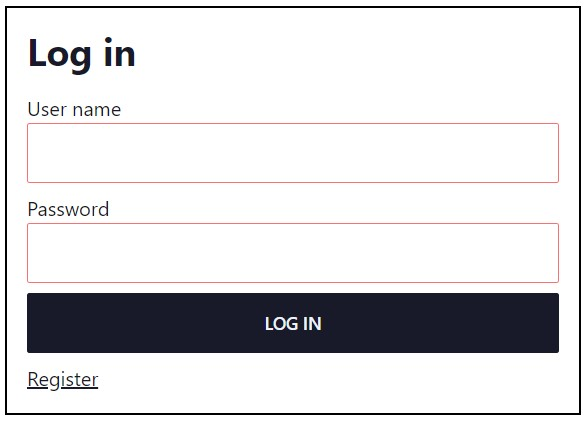
\includegraphics[width=10cm]{images/login.jpg}
\caption{Ekran prijave u sustav}
\label{fig:login}
\end{figure}

Ako korsnik unese neispravo koriničko ime ili ako predana zaporka nije točna za dano korisničko ime, onda sustav prikaže grešku gdje se navodi da nije ispravno korisničko ime ili zaporka, ali se ne kaže korisniku što točno nije ispravno.
Ako korisnik upiše ispravno korisničko ime i zaporku onda mu se dodijeli kolačić sjednice\footnote{https://www.cookieyes.com/blog/session-cookies/} i prebaci ga se na početnu stranicu aplikacije.
Kolačić sjednice se koristi da bi se nadalje znalo jeli korisnik autentifician i tko je korisnik.

Korisnik koji nema napravljen korisnički račun može prijeći na stranicu registracije preko poveznice na dnu komponente za prijavu.
Za uspješnu registraciju se od korisnika traži ime, prezime, korisničko ime te zaporku. Zaporka se mora dva puta unijeti te ako dvije unesene zaporke nisu jednake onda se korisniku ne dopušta predavanje unesenih podataka.

\begin{figure}[htb]
\centering
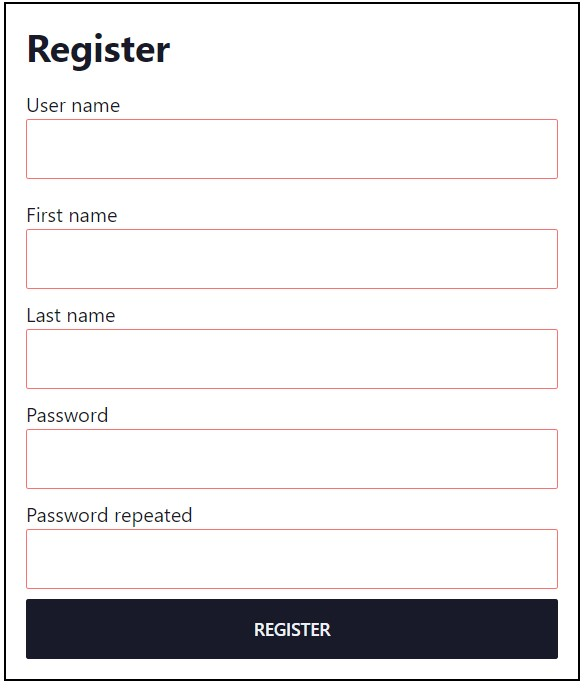
\includegraphics[width=10cm]{images/register.jpg}
\caption{Ekran registracije korisnika}
\label{fig:register}
\end{figure}

Ako korisnik unese korisničko ime koje se već koristi, onda mu korisničko sučelje prikaže da nije ispravno te da unese novo korisničko ime.
Ako su svi podatci ispravni, onda se nakon registracije automatski provede i prijava u sustav te se prebaci korisnika na početnu stranicu.

\section{Početna stranica}

TODO: Ovaj dio treba još prepraviti. Treba napraviti da prikazane utakmice se čitaju iz baze.

\section{Pregled utakmica}

Korisnik može doći do stranice pregleda utakmice preko navigacijske trake.

Prilikom dolaska na tu stranicu, od korisnika se traži da unese datum za koji želi pregledati utakmice. Ako korisnik nije ništa unio onda se automatski odabere datum posjećivanja stranice.
Nakon što korisnik unese željeni datum, aplikacija prikaže popis utakmice koje su igrane toga datuma uz osnovne informacije o tim utakmicama. Prikaže se ekipe koje su sudjelovale, datum i vrijeme igranja te rezultat.

\begin{figure}[htb]
\centering
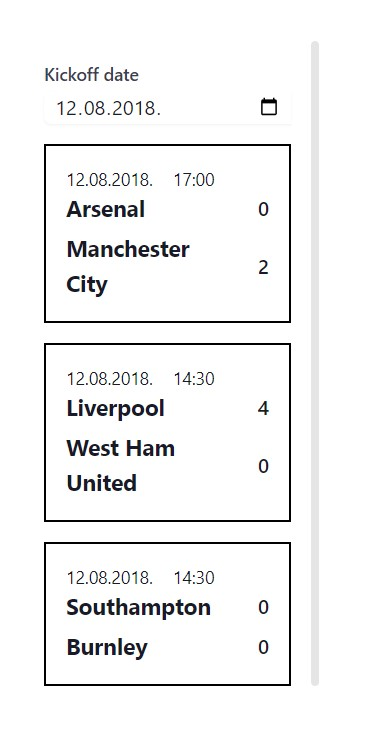
\includegraphics[width=5cm]{images/game-list.jpg}
\caption{Popis utakmica određenog datuma}
\label{fig:games-list}
\end{figure}

\subsection{Pregled detalja utakmice}

Nakon što korisnik odabere određenu utakmicu aplikacija će prikazati detalje te utakmice s desne strane popisa utakmica.
Stranica pregleda utakmica je napravljena koristeći ugniježđeno usmjeravanje (eng. nested routing)\footnote{https://start.solidjs.com/core-concepts/routing#nested-routes}.
To znači da prilikom promjene putanje unutar aplikacije ne radimo ponovno crtanje cijelog ekrana niti učitavamo sve podatke potrebne za cijelu stranicu.
Učitavamo samo podatke koji su potrebni za prikaz onih dijelova aplikacije koji se nalaze u promijenjenom segmentu putanje.
Na stranici pregleda detalja utakmice, aplikacije ima četiri razine ugniježđenog usmjeravanja. Prva razina se učitava za cijelu aplikaciju i ona sadrži samo navigacijsku traku i potake o tome jeli korisnik prijavljen i koju ulogu ima.
Druga razina se učitava kada se posjeti "/goals" putanju. Ta razina učitava popis dostupnih utakmica za dani datum i prikazuje ih s desne strane.
Treča razina sadrži identifikator utakmice. Tu se učitavaju osnvni podatci utakmice kao ime natjecanja i sezone u kojoj se igra utakmica, datum igranja, imena klubova, sličice grbova te rezultat.
Četvrta razina odabire jednu od tri kartice pregleda detalja utakmica: kartica s golovima, kartonima i zamjenama; kartica s grafičkim prikazom početnih jedanaest obje ekipe te kartica s statistikom utakmice.


Ako se ne odabere niti jedna kartica na četvrtoj razini, onda aplikacija automatski prebaci korisnika na karticu s golovima.

\begin{figure}[htb]
\centering
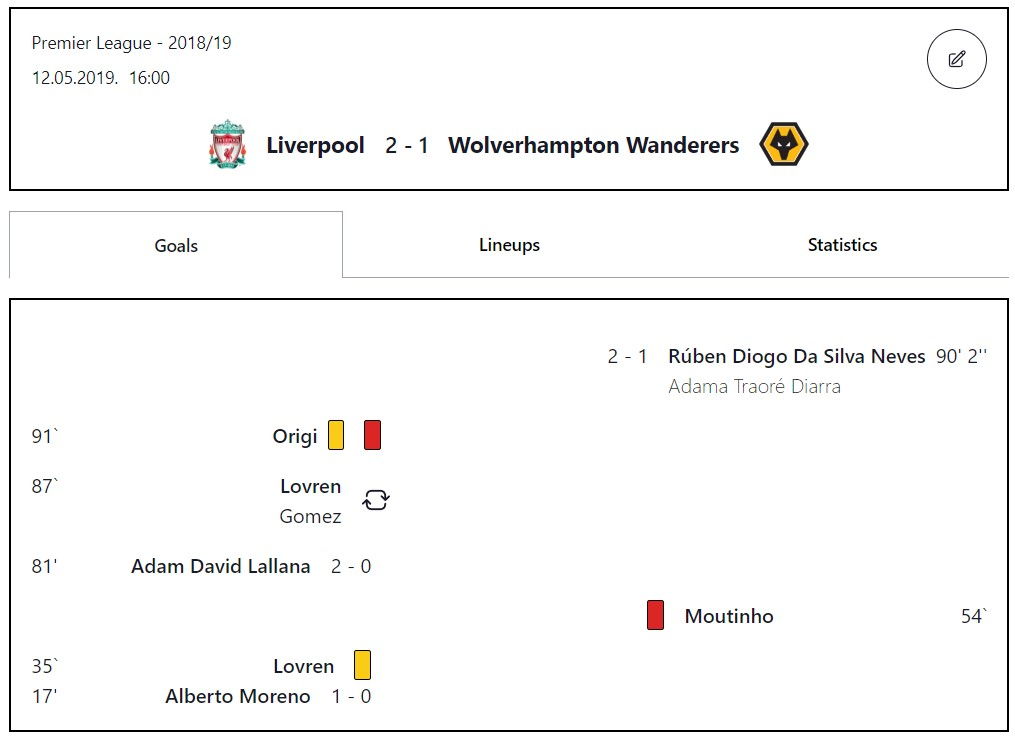
\includegraphics[width=15cm]{images/goals.jpg}
\caption{Osnovni podatci utakmice i popis golova}
\label{fig:goals}
\end{figure}

\subsection{Grafički prikaz početnih jedanaest}

Svaka spremljena utakmica mora imati spremljene podatke o početnih jedanaest obije ekipe.
Ekipa može imati jednu od sljedećih početnih formacija: 442, 433, 4231, 352, 3511, 343 i 532.
Na osnovu ovog podatka te spremljenih podataka u bazi podataka grafički se prikaže izgled početnih jedanaest.

\begin{figure}[htb]
\centering
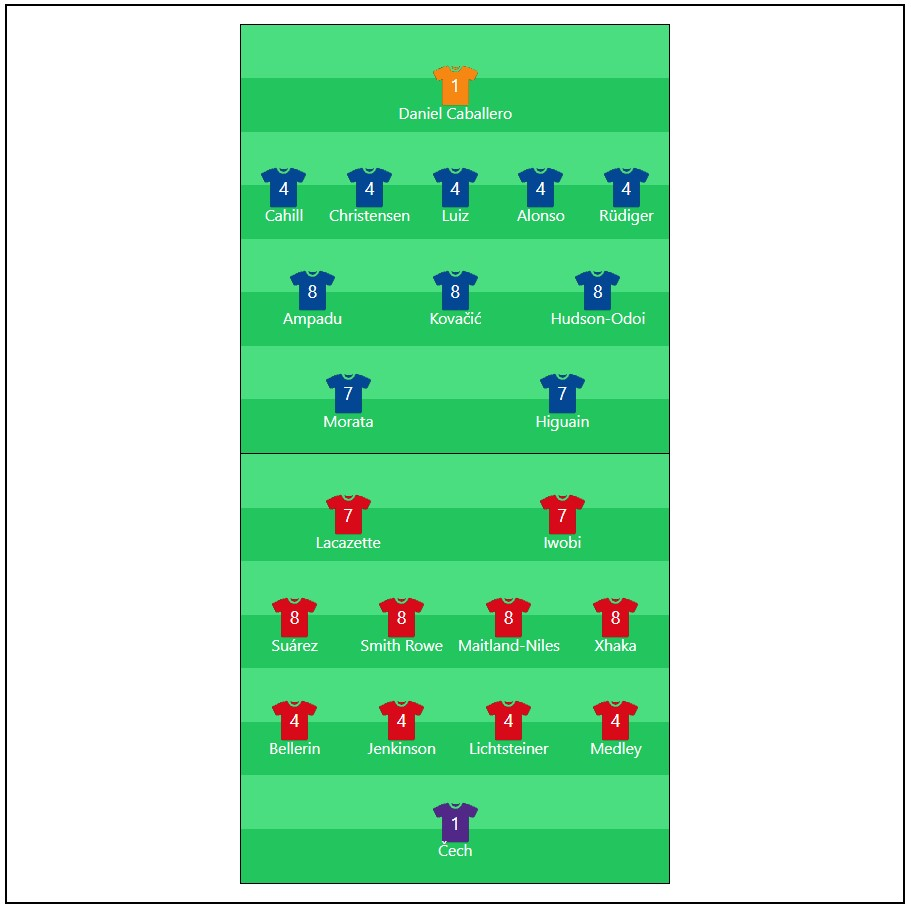
\includegraphics[width=15cm]{images/formation.jpg}
\caption{Početnih jedanaest}
\label{fig:formation}
\end{figure}

Za izradu ovog grafičkog prikaza je korišten samo CSS framework Tailwind\footnote{https://tailwindcss.com}.
Svi vidljivi elemti su ručno programirani koristeći samo dostupne tehnologije HTML-a i CSS-a. Oblik dresa je preuzet s interneta u SVG formatu te modificiran da se može mijenjati boja dresa ovisno o ekipi.
Prilikom klika ne jednog od igrača, korisnika se odvede na stranicu pregleda detalja tog igrača.

\subsection{Prikaz statistike}

Na stranici prikaza statistike prikazuju se podatci o posjedu lopte, ukupnim udarcima, udarcima u vrata, dodavanjima, ubačajima iz kuta, driblinzima, uspješnim driblimzima, zaleđima i sl.
Osim samog broja za odgovarajuću statistiku također se grafički prikazuju omjeer domaće i gostujuće ekipe.

\begin{figure}[htb]
\centering
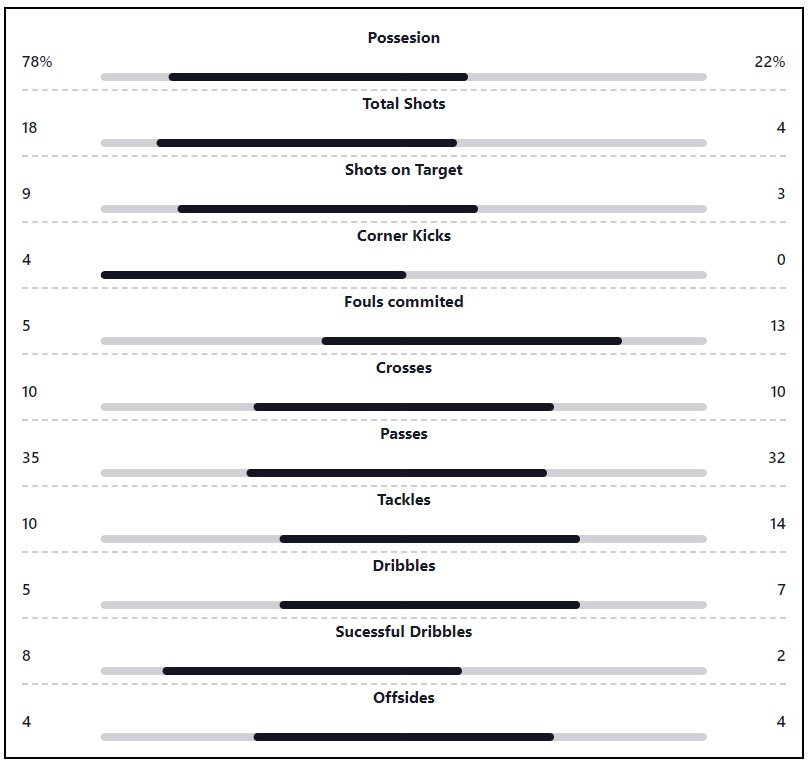
\includegraphics[width=15cm]{images/statistic.jpg}
\caption{Statistika utakmice}
\label{fig:statistic}
\end{figure}

\chapter{Zaključak}
Zaključak.

\bibliography{literatura}
\bibliographystyle{fer}

\begin{sazetak}
Ukratko opisati najznačajnije mogućnosti odabranih postojećih aplikacija namijenjenih prikazu statističkih
podataka o nogometnim utakmicama. Oblikovati relacijski model baze podataka za praćenje relevantnih
podataka o klubovima, igračima, sudjelovanju igrača u utakmicama, formacijama, rangu natjecanja,
zamjenama, trenerima ili izbornicima, posjedu lopte, asistencijama, udarcima u vrata i slično. Na osnovi
izgrađenog modela implementirati bazu podataka i web-aplikaciju za prikupljanje podataka i prikaz obrađenih
podataka o utakmicama, klubovima i igračima u prikladnom korisničkom sučelju. Za odabrani skup prikazanih
podataka osigurati osvježavanje podataka u korisničkom sučelju u stvarnom vremenu.

\kljucnerijeci{Ključne riječi, odvojene zarezima.}
\end{sazetak}

% TODO: Navedite naslov na engleskom jeziku.
\engtitle{Title}
\begin{abstract}
Abstract.

\keywords{Keywords.}
\end{abstract}

\end{document}
